\chapter{FlexTouch Working Principles}

\section{Sensing Principle of Touchscreen}
Most touch screens today are based on either self or mutual capacitive touch sensing. The mutual capacitive touch sensing method is widely adopted in industry due to its robustness in sensing multiple touch points simultaneously ~\cite{ye2015high}. The touch panel consists of multiple layers above the display screen as demonstrated in Figure ~\ref{fig:multi-layer-touchscreen}. A substrate glass etched with the sensing lines is attached. Then a layer of insulating material etched with the driving lines is placed on top. Finally, a bonding layer and a protective layer are placed on the top of the stack. 

The driving and sensing lines are made by a highly transparent conductive material named Indium Tin Oxide (ITO). They are oriented in a row-column matrix. A thin insulating layer between the driving lines and sensing lines forms a gap, the coupling mutual capacitance is formed at each junction (intersection between the driving and sensing lines) ~\cite{barrett2010projected}. Dedicated IC drives each driving line (row) and scans all the the sensing lines (columns) to measure the capacitance value at each row-column intersection. This procedure is repeated for all the driving lines as one entire cycle as Figure ~\ref{fig:touchscreen-principle-circuit} A) shows. 

\begin{figure}[h]
\centering
  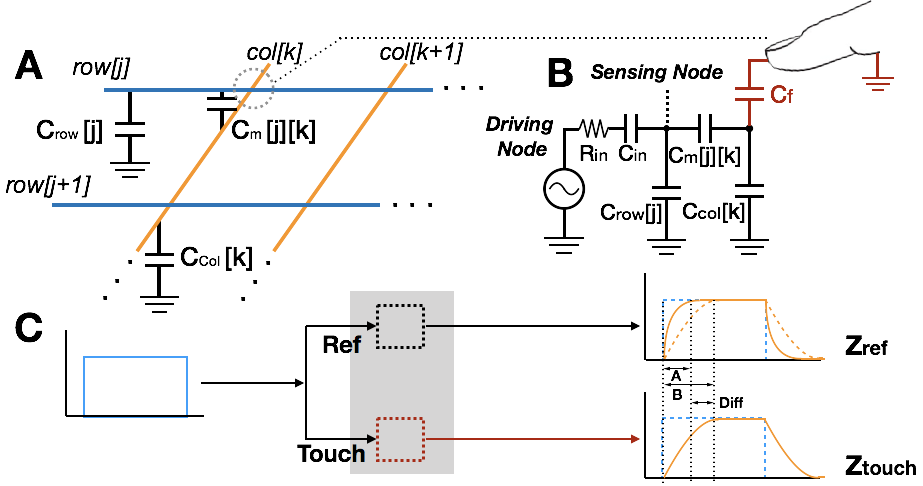
\includegraphics[width=0.95\columnwidth]{figures/touchscreen-principle-circuit.png}
  \caption{A: Representation of capacitive sensing row-column matrix structure B: Equivalent circuit of each junction. C: The measurement of capacitance of each junction.}
  \label{fig:touchscreen-principle-circuit}
\end{figure}

The finger touch increases the mutual capacitance of the touched electrodes. To detect the touch events, the driver IC measures the capacitance of each electrode intersection by comparing the source signal injected to the driving line and returned signal from the sensing line. The equivalent circuit and measuring method are illustrated in Figure ~\ref{fig:touchscreen-principle-circuit} B) and C). The standard method to detect the mutual capacitance of each junction is to measure the charging time to reach a certain voltage threshold between the driving line and the sensing line. 

\section{FlexTouch}

\textit{FlexTouch} extends the capacitive sensing method of commercially available touch screen to surrounding areas through a single conductive thread or frame attached on each sensing electrode. The attached conductive material, changes the electric field around the capacitive sensing junction. In this section, we explain the working principle, implementation and various of design configurations of \textit{FlexTouch}.

The conductive thread attached onto the touch screen draws currents passing from the driving line around the corresponding junctions. As a result, it takes more time to charge both the inner circuit and the attached conductive thread. In other words, any attached conductive material increases the mutual capacitance of the capacitive sensing node. Consider another case when people touch on the conductive thread, human body draws additional currents from the touch screen that further increases the mutual capacitance. In Figure ~\ref{fig:flextouch-principle-circuit} ,the measurement output from each junction node is positively correlated to mutual capacitance. In Figure  ~\ref{fig:flextouch-principle-circuit}A, the measurement of junction \#16 is 2 when no finger touch is present and now conductive thread is attached. When we connect an copper conductive thread onto the sensing node, the measurement jumped up to 983. And when a user is pressing onto the thread, the measurement is further increased to 1090 accordingly. If user press on both signal strip and grounding strip, the signal significantly increase to 1453, which demonstrated the amplifying effect of grounding strip.

Any conductive object in contact with the touchscreen draws currents passing from the driving line (transmitting electrode) to the sensing line (receiving electrode) at each junction. The control IC of the touchscreen is designed to measure this leaking current to detect touch events. Prior work introduced an extension tape enlarging the transmitting electrode to boost the touch sensing distance ~\cite{Kato2015, Kato2015a,mobicom-gao18, Ikematsu-Ohmic-Touch}. In Kato's work, the signal transmitted into the conductive tape returns to the device through an environmental coupling path, called \textbf{\textit{virtual ground}}. To further extend the capacitive sensing distance, we introduce the ground of the phone, the \textbf{\textit{local ground}}, into the extended circuit. Therefore, we can short this coupling path with another conductive tape directly passing the signal back to the touchscreen device. Although the local ground can be extended from the charging port, we use the back panel of the touchscreen device since it's easier to assemble as illustrated in Fig ~\ref{fig:plugandplay} C. We can simplify the structure made of the attached conductive tape, the back panel, and the inner local ground circuit as one large capacitor. Here, we define two types of extension strips: 1) \textbf{\textit{signal strip}}, which is attached to the touchscreen sensor node, and 2) \textbf{\textit{grounding strip}} which extends the local ground of the touchscreen.

\begin{figure}[ht]
\centering
    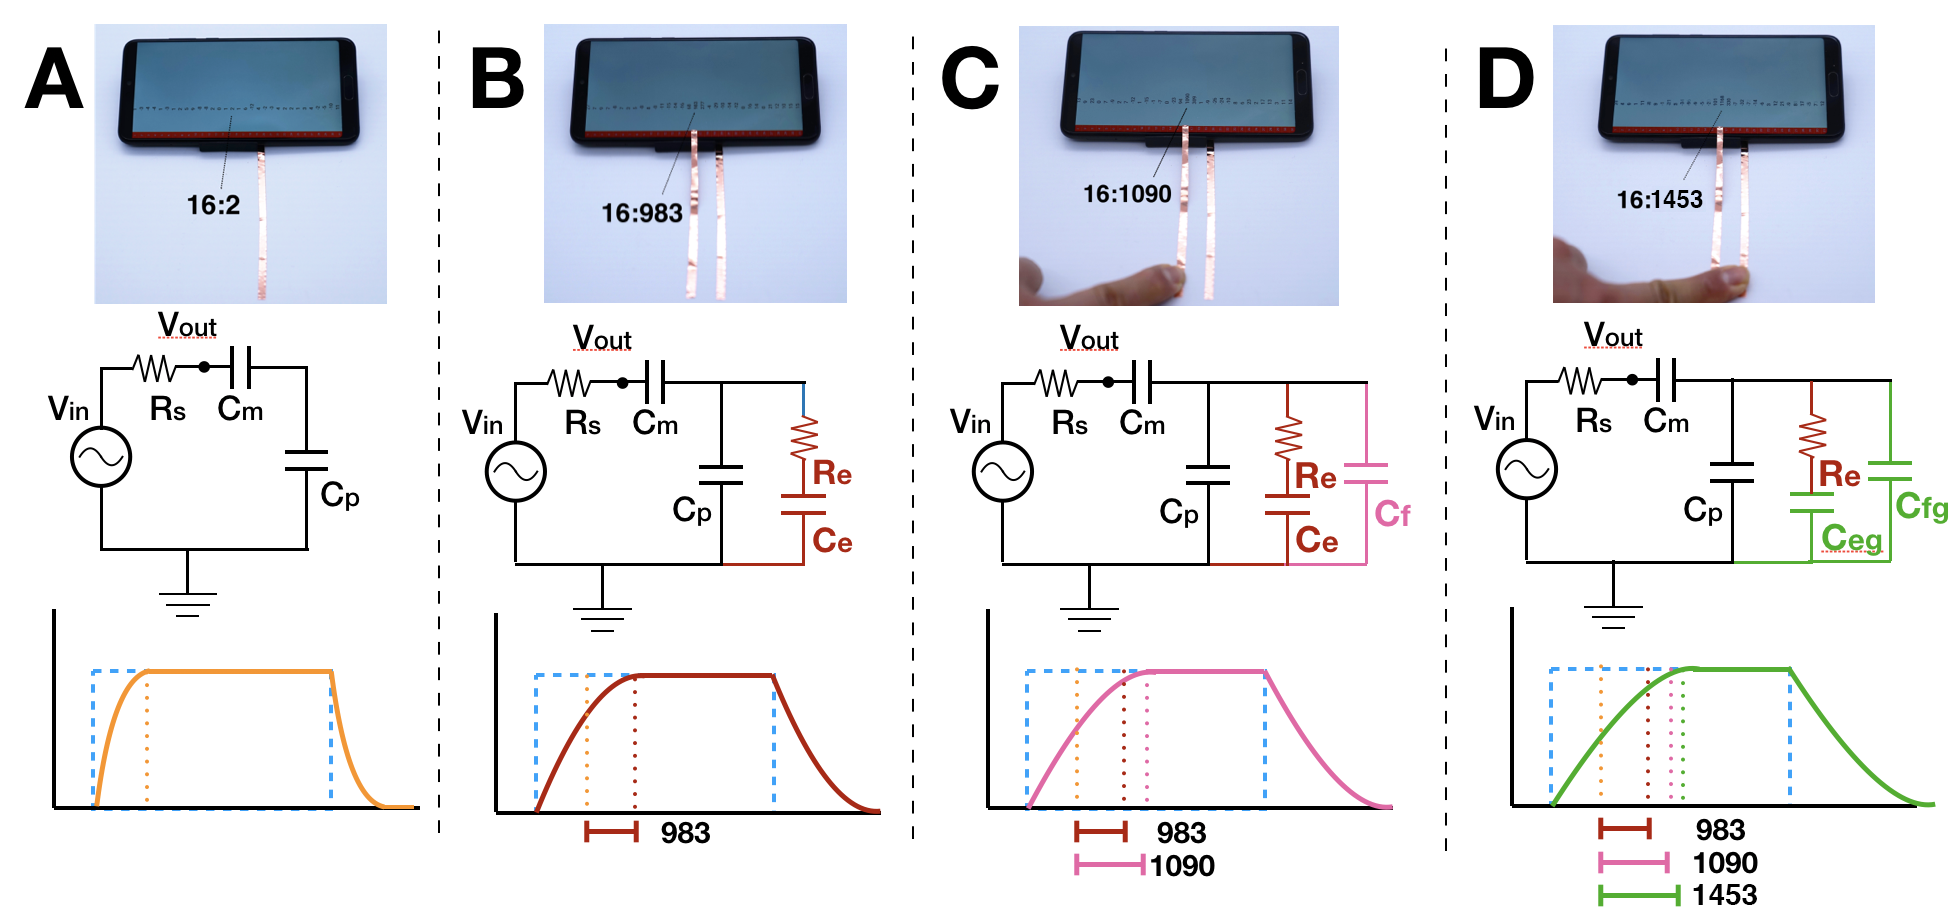
\includegraphics[width=0.95\columnwidth]{figures/flextouch-principle-circuit.png}
    \setlength{\belowcaptionskip}{-6pt}
    \caption{Four capacitive states and corresponding simplified equivalent circuits of \textit{FlexTouch}. A: Idle state - original touchscreen sensing node. B: Attaching state - adding the signal strip on one touchscreen sensing node. C: Touching state - touch on the signal strip. D: Grounding state - touch both the signal strip and the grounding strip.}
    \label{fig:flextouch-principle-circuit}
\end{figure}

We present simplified equivalent circuits under each column in Fig ~\ref{fig:flextouch-principle-circuit} with each capacitive sensor node treated as a RC circuit. $R_{s}$, $C_{m}$, $C_{p}$, $C_{e}$, $C_{f}$, $C_{fg}$,$C_{eg}$, $R_{e}$ represent the inner resistance, mutual capacitance, parasitic capacitance, introduced capacitance between the extended element and local ground, touch introduced capacitance, introduced capacitance of touching both the signal and grounding strips, changed capacitance between the extended element and local ground as well as the extended element introduced resistance. Equation (1) shows the calculation of $v_{out}$ ignoring the effect of $R_{e}$, using $C_{e(g)}$ representing either $C_{e}$ or $C_{eg}$ and $C_{f(g)}$ representing either $C_{f}$ or $C_{fg}$.

\begin{equation}
    V_{out} = v_{in}(1-e^{-\frac{C_{m} + C_{p} + C_{e(g)} + C_{f(g)}}{R_{s}C_{m}(C_{p} + C_{e(g)} + C_{f(g)})}t})
\end{equation}


The touchscreen controller transmits a series of step voltage signals to scan through each electrode and measures the charging time (time for $V_{out}$ to reach a threshold) as raw capacitive values of the touchscreen. The charging time is linearly dependent on the Time Constant of the RC circuit, named $\tau$, that is given as:

\begin{equation}
    \tau = R_{s}\frac{C_{m}(C_{p} + C_{e(g)} + C_{f(g)})}{C_{m} + C_{p} + C_{e(g)} + C_{f(g)}}
\end{equation}

 
We assume that $C_{m}$ and $C_{p}$ are static with value around $10pF$. The value of $C_{e}$ depends on the characteristics of the extended surfaces such as conductivity of the material, length, and width as well as the intersection effect between the extended elements. $C_{f}$ typically varies from several to dozens of $pF$ introduced by human touch. 

Fully understanding the effect of $C_{e}$ is the key to exploring the upper-limit of \textit{FlexTouch}'s performance. In pursuit of testing this limit, we simply model the mutual capacitance between the extended material and the virtual ground with following formula.

\begin{equation}
    C_{e} = \varepsilon \frac{A}{d} = \varepsilon \frac{L \times D}{d}
\end{equation}

$A$ represents the scale of dimensions of extension strips including length ($L$) and width ($D$), $d$ represents the separation between the signal strip and the local ground, and $\varepsilon$ represents the material's permittivity of extension strips. Therefore, to fully evaluate the sensing distance capability of \textit{FlexTouch}, we need to study the effect of variable factors contained in the fabrication material along with the width and gap distance of the extension strips.